\chapter{تنوع الكائنات وحيدة الخلية}\label{ch:b2:unicellular-diversity}

قطرة من ماء بركة تحت المجهر تضم خلية خضراء تجدّف بسوطين، وهدبيًا على
شكل نعل يكنس البكتيريا إلى بلعومه، ودياتومًا زجاجيًا ينزلق على
الشريحة، وألف بكتيريا أصغر من أن تُرى جيدًا. كل واحد منها خلية واحدة
وكائن حي كامل في آن: يتغذى ويتحرك ويحسّ وينمو ويتكاثر ويموت وهو خلية
مفردة. وهكذا كان جل العالم الحي على الدوام. يتناول هذا الفصل \omterm{def:b2:unicellular-diversity:unicellular}{الكائن
وحيد الخلية} بوصفه مسألة تصميم --- ما تستطيعه خلية واحدة وما لا
تستطيعه --- ويستعرض الأجوبة التي وجدتها بدائيات النوى وحقيقيات
النوى، إلى الحد الذي تبدأ عنده الخلايا في البقاء معًا.

\section{خلية واحدة، وكل الوظائف}

\begin{definition}[وحيد الخلية، مستعمري، عديد الخلايا]\label{def:b2:unicellular-diversity:unicellular}
يكون الكائن \emph{وحيد الخلية}\index{كائن وحيد الخلية} حين تؤدي خلية
واحدة كل وظائف الحياة --- التغذية والتبادل والحركة والتكاثر ---
وتعيش بذاتها. ويكون \emph{مستعمريًا}\index{كائن مستعمري} حين تبقى
خلايا من نوع واحد ملتصقة بعد انقسامها، مع بقاء كل منها قادرة على
العيش وحدها لو فُصلت. ويكون \emph{عديد الخلايا}\index{كائن عديد الخلايا}
حين تكون خلاياه من أنواع عدة يعتمد بعضها على بعض، ولا يخلّف نسلًا منها إلا قليل (السلالة الجنسية). وتشمل الكائنات وحيدة
الخلية العتائق كلها، وجل البكتيريا، ومعظم سلالات حقيقيات النوى؛
والاسم غير الاصطلاحي \emph{\omterm{def:b2:unicellular-diversity:protist}{الطلائعيات}} يغطي حقيقيات النوى وحيدة
الخلية، وهي ليست مجموعة واحدة بل مجموعات كثيرة.
\end{definition}

\begin{example}[ستة من سكان القطرة]\label{ex:b2:unicellular-diversity:drop}
\emph{Escherichia coli} عصية طولها \qty{2}{\micro m}، تسبح بخصلة من
الأسواط وتنقسم كل عشرين دقيقة متى وجدت الغذاء.
و\emph{Chlamydomonas} طحلب أخضر قطره \qty{10}{\micro m}، يجدّف
بسوطين نحو الضوء الذي يكشفه ببقعة عينية. و\emph{Paramecium} هدبي
قياسه \qty{200}{\micro m}، يغطيه آلاف الأهداب، ويتغذى عبر بلعوم،
ويطرح الماء بفجوتين متقلصتين. والدياتوم يعيش في قوقعة سيليسية من
شطرين مزخرفة بالمسام. و\emph{Amoeba} تسيل بمدّ أقدام كاذبة وتبتلع
ما تلقاه. وخلية الخميرة تُبرعم بنتًا من جنبها. ستة أجوبة، شديدة
الاختلاف في القياس والآلات، عن مسألة واحدة.
\end{example}

\begin{omfigure}
\begin{tikzpicture}[x=1.9cm]
  % log scale from 0.1 um to 100 mm : position = log10(size in um) + 1
  \draw[thick] (0,0) -- (6,0);
  \foreach \p/\l in {0/{\qty{0.1}{\micro m}},1/{\qty{1}{\micro m}},2/{\qty{10}{\micro m}},3/{\qty{100}{\micro m}},4/{\qty{1}{mm}},5/{\qty{10}{mm}},6/{\qty{100}{mm}}}
    \draw (\p,0.12) -- (\p,-0.12) node[below, font=\scriptsize] {\l};
  \foreach \p/\c/\l in {0.5/omDef/{ميكوبلازما}, 1.3/omDef/{\emph{E.~coli}}, 1.7/omDef/{خميرة}, 2.0/omProp/{\emph{Chlamydomonas}}, 2.7/omProp/{دياتومات}, 3.3/omProp/{\emph{Paramecium}}, 3.65/omProp/{\emph{Amoeba proteus}}, 3.9/omThm/{\emph{Thiomargarita} (بكتيريا)}, 5.7/omProp/{\emph{Acetabularia}}}
    { \fill[\c] (\p,0) circle (0.05); \node[rotate=60, anchor=west, font=\scriptsize, \c, inner sep=1pt] at (\p,0.12) {\l}; }
  \node[font=\scriptsize, anchor=north] at (3,-0.55) {قياس الخلية (سلم لوغاريتمي)};
\end{tikzpicture}

{\small تمتد قياسات الكائنات وحيدة الخلية على خمس رتب من القدر.
بدائيات النوى (بالأزرق) تتجمع حول الميكرومتر؛ وخلايا حقيقيات النوى
(بالبرتقالي) أكبر منها بعشر إلى مئة مرة؛ أما أكبر الخلايا المفردة
--- بكتيريا كبريتية عملاقة، والطحلب \emph{Acetabularia} ---
فاستثناءات يشرحها النص.}
\end{omfigure}

\begin{proposition}[السطح والحجم والحد على القياس]\label{prop:b2:unicellular-diversity:surface}
\index{نسبة السطح إلى الحجم}
تتبادل الخلية مع محيطها عبر سطحها وتستهلك بنسبة حجمها. ومن أجل كرة
نصف قطرها $r$، تكون \emph{\omterm{prop:b2:unicellular-diversity:surface}{نسبة السطح إلى الحجم}}
\[
\frac{S}{V} = \frac{4\pi r^2}{\tfrac{4}{3}\pi r^3} = \frac{3}{r},
\]
أي إن مضاعفة نصف القطر تنصّف السطح المتاح لكل وحدة من السيتوبلازم.
ولذلك لا تستطيع خلية تعتمد على الانتشار عبر غشائها في تغذية داخلها
أن تنمو بلا حد: فعند نصف قطر ما لا يعود الوارد عبر السطح يلبي طلب
الحجم. والقانون نفسه يفسر لماذا تكون الخلايا الصغيرة أنشط استقلابيًا
لكل غرام، ولماذا تكون الخلايا الكبيرة مفلطحة أو مستطيلة أو مفجَّوة
أو مملوءة بأغشية داخلية.
\end{proposition}

\begin{theorem}[زمن الانتشار عبر مسافة]\label{thm:b2:unicellular-diversity:diffusion}
\index{زمن الانتشار}
جزيئة معامل انتشارها $D$ تهيم في خطوات عشوائية؛ وبعد زمن $t$ يكون
متوسط مربع انزياحها على محور واحد $\langle x^2\rangle = 2Dt$. ومن ثم
يكون الزمن اللازم لقطع مسافة $x$ بالانتشار وحده
\[
t \approx \frac{x^2}{2D},
\]
وهو ينمو مع \emph{مربع} المسافة. فمع $D \approx \qty{1e-9}{m^2/s}$
لجزيئة صغيرة في الماء، يستغرق عبور بكتيريا (\qty{1}{\micro m}) نصف
ميلي ثانية؛ أما عبور خلية قياسها \qty{1}{mm} فيستغرق ثماني دقائق،
وعبور متر واحد ستة عشر عامًا.
\end{theorem}
\begin{proof}
لتخطُ الجزيئة خطوات طولها $\ell$ يمينًا أو يسارًا عشوائيًا كل $\tau$
ثانية. بعد $n$ خطوة يكون انزياحها $x = \sum_i \varepsilon_i \ell$ مع
$\varepsilon_i = \pm 1$ مستقلة، ومن ثم $\langle x\rangle = 0$
و$\langle x^2\rangle =
\sum_i \langle\varepsilon_i^2\rangle \ell^2 = n\ell^2$ (إذ تتلاشى
الحدود المتقاطعة في المتوسط). وبوضع $n = t/\tau$ يصير هذا $\langle x^2\rangle
= (\ell^2/\tau)\,t$، وبكتابة $D = \ell^2/2\tau$ نجد
$\langle x^2\rangle = 2Dt$. ووضع $\langle x^2\rangle = x^2$ يعطي
الزمن المطلوب.
\end{proof}

\begin{theorem}[الوارد بالانتشار إلى خلية كروية]\label{thm:b2:unicellular-diversity:supply}
\index{الاقتناء المحدود بالانتشار}
خلية كروية نصف قطرها $r_0$ تمتص كل جزيئة من مادة منحلّة تبلغ سطحها،
في وسط يكون فيه التركيز البعيد $c_\infty$، تتلقى في الحالة
المستقرة تدفقًا (جزيئات في الثانية) قدره
\[
J = 4\pi D r_0\, c_\infty .
\]
ينمو الوارد مع $r_0$ وحدها، بينما ينمو الطلب مع $r_0^3$: فوراء نصف
قطر معين تجوع خلية تتغذى بالانتشار.
\end{theorem}
\begin{proof}
في الحالة المستقرة يكون عدد الجزيئات التي تعبر كل كرة نصف قطرها
$r > r_0$ في الثانية واحدًا، أي $J = 4\pi r^2 D\,
(\mathrm{d}c/\mathrm{d}r)$ (قانون فيك، والتدفق موجّه إلى الداخل).
فيكون $r^2\,\mathrm{d}c/\mathrm{d}r = J/4\pi D$ ثابتًا؛ وبالمكاملة
من $r_0$، حيث $c = 0$، إلى اللانهاية، حيث $c = c_\infty$، نجد
$c_\infty = (J/4\pi D)\int_{r_0}^{\infty} r^{-2}\,\mathrm{d}r =
J/(4\pi D r_0)$، ومنه $J = 4\pi D r_0 c_\infty$.
\end{proof}

\begin{example}[ما أكبر خلية تتغذى بالانتشار؟]\label{ex:b2:unicellular-diversity:howbig}
تستهلك خلية هوائية الأكسجين بمعدل نحو $q = \qty{0.02}{mol/m^3/s}$
من السيتوبلازم (معدل نشيط). وطلبها هو $q \cdot \tfrac{4}{3}\pi
r_0^3$؛ أما الوارد من ماء مشبع بالهواء ($c_\infty =
\qty{0.25}{mol/m^3}$، $D = \qty{2e-9}{m^2/s}$) فهو $4\pi D r_0
c_\infty$. وبالمساواة، $r_0^2 = 3Dc_\infty/q = 3\times 2\times 10^{-9}
\times 0.25/0.02 = \qty{7.5e-8}{m^2}$، ومنه $r_0 \approx
\qty{270}{\micro m}$. وتبقى الخلايا النشيطة الحقيقية دون ذلك بكثير
لأن على الأكسجين أن ينتشر \emph{داخلها} أيضًا؛ والبكتيريا الكبريتية
\emph{Thiomargarita} التي قياسها \qty{750}{\micro m} تلتف على الحد
بكونها فجوة كلها تقريبًا، وسيتوبلازمها قشرة رقيقة لا يتجاوز عمقها
بضعة ميكرومترات.
\end{example}

\begin{omfigure}
\begin{tikzpicture}
\begin{axis}[
  width=0.8\linewidth, height=6.2cm,
  axis x line=bottom, axis y line=left,
  xmode=log, ymode=log,
  xmin=0.3, xmax=1000, ymin=1e-6, ymax=1e4,
  xlabel={نصف قطر الخلية (\unit{\micro m})}, ylabel={جزيئات في الثانية (نسبيًا)},
  xlabel style={font=\small, at={(axis description cs:0.5,-0.1)}, anchor=north},
  ylabel style={font=\small},
  tick label style={font=\small},
  legend style={font=\small, at={(0.03,0.97)}, anchor=north west, draw=none},
  clip=false,
]
\addplot[very thick, omDef, domain=0.3:1000, samples=40] {x/10};
\addlegendentry{الوارد بالانتشار، $\propto r$}
\addplot[very thick, omThm, domain=0.3:1000, samples=40] {(x/10)^3/1000*1.0};
\addlegendentry{طلب السيتوبلازم، $\propto r^3$}
\draw[dashed, gray] (axis cs:270,1e-6) -- (axis cs:270,27);
\node[font=\scriptsize, anchor=west] at (axis cs:300,3e-4) {نصف قطر التجويع};
\end{axis}
\end{tikzpicture}

{\small ينمو الوارد عبر السطح مع $r$، وينمو الطلب مع
$r^3$ (محاور لوغاريتمية). وحيث يتقاطع الخطان لا تعود الخلية التي
تتغذى بالانتشار وحده قادرة على إمداد داخلها؛ ويقع التقاطع قرب بضع
مئات من الميكرومترات عند خلية هوائية نشيطة.}
\end{omfigure}

\section{تنوع بدائيات النوى}

\begin{definition}[الخلية بدائية النواة]\label{def:b2:unicellular-diversity:prokaryote}
\emph{بدائي النواة}\index{بدائي النواة} (البكتيريا والعتائق، وهما
مجالان متباعدان أحدهما عن الآخر تباعد كل منهما عنا) خلية بلا نواة
ولا عضيات محاطة بأغشية: صبغي حلقي واحد في
\emph{جسم نووي}\index{جسم نووي}، وغالبًا معه حلقات صغيرة إضافية
تسمى \emph{البلازميدات}\index{بلازميد}، وريبوزومات حرة في
سيتوبلازم قياسه \qtyrange{0.5}{2}{\micro m}، وغشاء هيولي يحمل
سلاسل التنفس أو التركيب الضوئي، و\emph{جدار خلوي}\index{جدار خلوي!بكتيري}
صلب يقاوم امتلاء سيتوبلازم يعلو محيطه ببضعة بارات.
والأشكال قليلة ولها أسماء: \emph{المكوّر} (كرة)، و\emph{العصية}
(قضيب)، و\emph{الملتوية} و\emph{اللولبية} (حلزونان)،
و\emph{الضمّة} (فاصلة)؛ وقد تبقى الخلايا أزواجًا أو سلاسل أو
رباعيات أو عناقيد بعد انقسامها.
\end{definition}

\begin{proposition}[غلافان: إيجابية غرام وسلبية غرام]\label{prop:b2:unicellular-diversity:gram}
\index{صبغة غرام}\index{الببتيدوغليكان}
يُبنى الجدار البكتيري من \emph{الببتيدوغليكان}، وهو سلاسل من سكرين
متناوبين تشابكها ببتيدات قصيرة في جزيئة عملاقة واحدة حول الخلية.
وللبكتيريا \emph{الإيجابية الغرام} طبقة سميكة
(\qtyrange{20}{80}{nm}) خارج غشاء واحد، تحتفظ بصبغة البنفسج
البلوري في طريقة غرام؛ أما البكتيريا \emph{السلبية الغرام} فلها
طبقة رقيقة (بضعة نانومترات) محصورة بين الغشاء الهيولي
و\emph{غشاء خارجي} وريقته الخارجية من عديد سكريد شحمي، وهي تفقد
الصبغة. والغشاء الخارجي، المثقوب ببوابات بروتينية، حاجز ثانٍ:
يصدّ كثيرًا من الصادات والمنظفات، ولذلك يصعب علاج أخماج سلبيات
الغرام. أما العتائق فلا ببتيدوغليكان لها ولا الشحوم الإستيرية التي
لكل خلية سواها: أغشيتها مبنية من سلاسل إيزوبرينية بروابط إيثيرية،
تمتد أحيانًا عبر الطبقة المضاعفة كلها فتصير طبقة واحدة، وهو ما
يبقيها ثابتة في حمض يغلي.
\end{proposition}

\begin{omfigure}
\begin{tikzpicture}[scale=0.9, every node/.style={font=\scriptsize}]
  % Gram-positive
  \begin{scope}
    \fill[omDef!15] (0,0) rectangle (4,1.6);
    \node at (2,0.4) {السيتوبلازم};
    \fill[omDef!60] (0,1.6) rectangle (4,1.85);
    \node[right] at (4.05,1.72) {غشاء هيولي};
    \fill[omProp!50] (0,1.85) rectangle (4,3.0);
    \foreach \y in {2.0,2.25,...,2.85} \draw[omProp!90!black] (0.1,\y) -- (3.9,\y);
    \node[right, align=left] at (4.05,2.45) {ببتيدوغليكان سميك\\(\qtyrange{20}{80}{nm})};
    \node[above, font=\small\bfseries] at (2,3.05) {إيجابية غرام};
  \end{scope}
  % Gram-negative
  \begin{scope}[xshift=7.6cm]
    \fill[omDef!15] (0,0) rectangle (4,1.6);
    \node at (2,0.4) {السيتوبلازم};
    \fill[omDef!60] (0,1.6) rectangle (4,1.85);
    \node[right] at (4.05,1.72) {غشاء هيولي};
    \fill[omProp!50] (0,2.05) rectangle (4,2.25);
    \draw[omProp!90!black] (0.1,2.15) -- (3.9,2.15);
    \node[right] at (4.05,2.15) {ببتيدوغليكان رقيق};
    \node at (2,1.95) {الفراغ المحيطي};
    \fill[omThm!50] (0,2.55) rectangle (4,2.85);
    \foreach \x in {0.6,2.0,3.4} \fill[white] (\x-0.12,2.55) rectangle (\x+0.12,2.85);
    \node[right] at (4.05,2.7) {غشاء خارجي ببوابات};
    \foreach \x in {0.2,0.5,...,3.9} \draw[omThm!80!black, thick] (\x,2.85) -- (\x,3.1);
    \node[right] at (4.05,3.15) {عديد سكريد شحمي};
    \node[above, font=\small\bfseries] at (2,3.3) {سلبية غرام};
  \end{scope}
\end{tikzpicture}

{\small الغلافان البكتيريان في مقطع. على اليمين: غشاء واحد تحت
كساء سميك من الببتيدوغليكان. وعلى اليسار: طبقة رقيقة من
الببتيدوغليكان في الفراغ المحيطي بين غشاءين، الخارجي منهما مرصّع
بالبوابات ومكسوّ بعديد السكريد الشحمي.}
\end{omfigure}

\begin{proposition}[السوط البكتيري والانجذاب الكيميائي]\label{prop:b2:unicellular-diversity:flagellum}
\index{سوط!بكتيري}\index{انجذاب كيميائي}
\emph{السوط} البكتيري خيط حلزوني صلب من بروتين الفلاجيلين، ثخنه
\qty{20}{nm} وطوله أضعاف طول الجسم، يديره محرك دوّار مركّب في
الغلاف. ولا يعمل المحرك بجزيئات ATP بل بالبروتونات المنحدرة مع التدرج
الكهركيميائي عبر الغشاء، بنحو \num{1000} بروتون في الدورة وحتى
\num{300} دورة في الثانية. وفي \emph{E.~coli} تتجمع الأسواط العديدة
في خصلة واحدة حين تدور كلها عكس عقارب الساعة، فتدفع الخلية في
\emph{شوط} مستقيم؛ وحين ينعكس واحد منها أو أكثر تتفكك الخصلة
\emph{فتتقلقل} الخلية إلى اتجاه عشوائي جديد. و\emph{\omterm{prop:b2:unicellular-diversity:flagellum}{الانجذاب
الكيميائي}} هو إمالة هذا المشي العشوائي: تقيس الخلية هل ارتفع تركيز
مادة جاذبة خلال الثانية الأخيرة، فإن ارتفع كبحت التقلقل. فهي توجّه
نفسها بمقارنة الحاضر بالماضي القريب --- على امتداد مسارها --- لأن
لا تدرج قابلًا للقياس عبر \qty{1}{\micro m} من طولها.
\end{proposition}
\begin{proof}[شواهد]
تابع بيرغ وبراون (1972) خلايا \emph{E.~coli} مفردة في ثلاثة أبعاد
بمجهر متعقّب: أشواط تدوم نحو ثانية بسرعة \qty{20}{\micro m/s}،
وتقلقلات تدوم عُشر ثانية، وفي تدرج من السيرين كانت الأشواط الصاعدة
مع التدرج أطول بينما لم تقصر الأشواط النازلة. وربط خلية إلى شريحة
زجاجية بسوط واحد جعل الجسم كله يدور، وهو ما أثبت أن المحرك دوّار؛
والخلايا التي فُصل محركها عن اصطناع ATP ظلت تسبح ما دام يمكن فرض
تدرج بروتوني، وهو ما عيّن الوقود.
\end{proof}

\begin{omfigure}
\begin{tikzpicture}[every node/.style={font=\scriptsize}]
  % run and tumble path without gradient
  \begin{scope}
    \draw[very thick, omDef] (0,0) -- (1.2,0.5) -- (0.7,1.4) -- (1.9,1.8) -- (2.6,0.9) -- (3.4,1.5) -- (3.0,2.5);
    \foreach \p in {(1.2,0.5),(0.7,1.4),(1.9,1.8),(2.6,0.9),(3.4,1.5)} \fill[omThm] \p circle (0.06);
    \node[align=center] at (1.8,-0.5) {بلا تدرج:\\أشواط متساوية الطول، ودورات عشوائية};
  \end{scope}
  \begin{scope}[xshift=6cm]
    \shade[left color=white, right color=omExo!50] (-0.3,-0.2) rectangle (5.2,3.0);
    \draw[very thick, omDef] (0,0.3) -- (0.9,0.8) -- (0.6,1.3) -- (2.4,1.5) -- (2.2,2.2) -- (4.6,2.4);
    \foreach \p in {(0.9,0.8),(0.6,1.3),(2.4,1.5),(2.2,2.2)} \fill[omThm] \p circle (0.06);
    \node[align=center] at (2.4,-0.5) {مادة جاذبة تتزايد نحو اليسار:\\الأشواط الصاعدة مع التدرج أطول};
    \node[anchor=south east] at (5.1,2.6) {مادة جاذبة أكثر};
  \end{scope}
\end{tikzpicture}

{\small الشوط والتقلقل. على اليمين: بلا تدرج تؤدي الخلية مشيًا
عشوائيًا، وينتهي كل شوط (بالأزرق) بتقلقل (نقطة حمراء). وعلى
اليسار: حين تتزايد مادة جاذبة على امتداد شوط، يُكبح التقلقل ويطول
الشوط؛ فينحرف المشي صاعدًا مع التدرج.}
\end{omfigure}

\begin{example}[الزراقم والخلية المغايرة]\label{ex:b2:unicellular-diversity:cyanobacteria}
الزراقم بكتيريا تركّب ضوئيًا كما تفعل النباتات، فتشق الماء وتطلق
الأكسجين على أغشية داخلية مكدّسة (الثايلاكويدات، التي ورثها عنها
الصانع الأخضر). وكثير منها ينمو خيوطًا من خلايا تتشارك غمدًا
واحدًا. وفي \emph{Anabaena}، حين ينفد النتروجين المؤتلف، تصير كل خلية
عاشرة تقريبًا \emph{خلية مغايرة}: تفكك جهازها الضوئي المنتج
للأكسجين، وتثخّن جدارها في وجه الأكسجين، وتثبّت نتروجين الجو بإنزيم
كان الأكسجين ليتلفه، وتصدّر الغلوتامين إلى جاراتها مقابل السكر.
وخيط \emph{Anabaena} رسم أول لتقسيم عمل بين الخلايا.
\end{example}

\begin{omfigure}
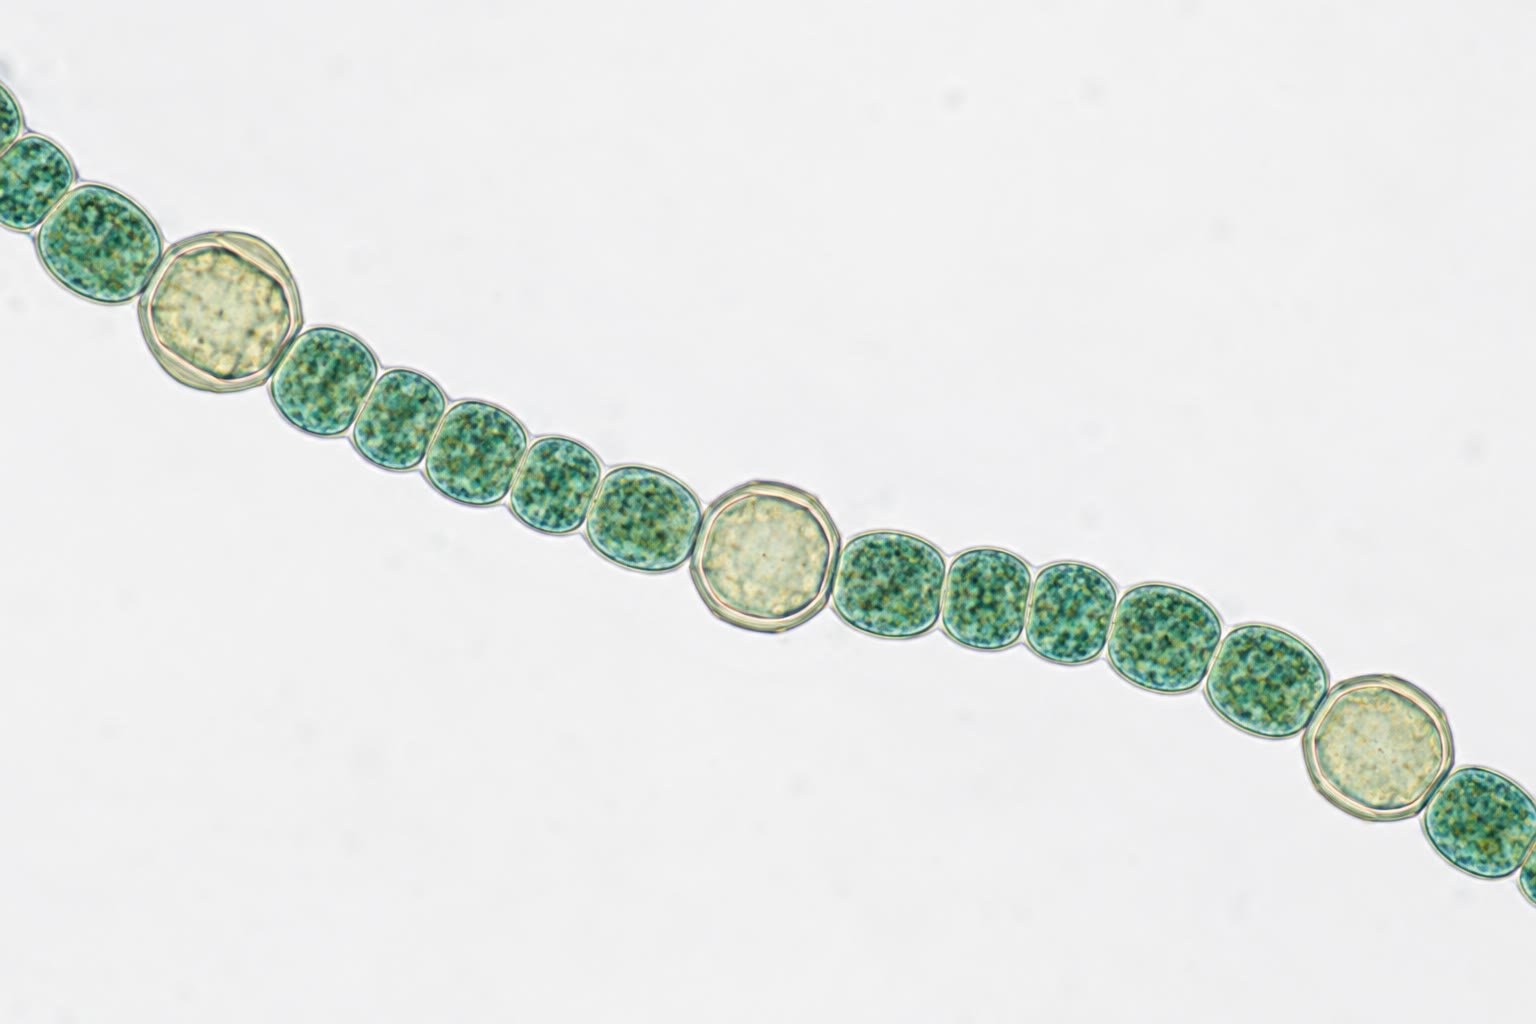
\includegraphics[width=0.62\linewidth]{images/book4/ai/b4-01-anabaena.jpg}

{\small خيط من \emph{Anabaena}: سلسلة من خلايا خضراء مركّبة ضوئيًا
تقطعها خلايا مغايرة أكبر وأشحب، وهي الخلايا التي تثبّت النتروجين.}
\end{omfigure}

\begin{remark}[السكون]\label{rem:b2:unicellular-diversity:spores}
تجيب بعض العصيات الإيجابية الغرام (\emph{Bacillus}،
\emph{Clostridium}) عن التجويع ببناء \emph{بوغ داخلي}: نسخة من
الصبغي ملفوفة في عدة أكسية منزوعة الماء، خاملة استقلابيًا، تقاوم
الغليان والإشعاع وقرونًا من الجفاف، وتنبت حين تعود الظروف. وكثير
من \omterm{def:b2:unicellular-diversity:protist}{الطلائعيات} يفعل الشيء نفسه \emph{بكيس}. والسكون هو الطريقة
الأخرى للنجاة من موسم رديء، إلى جانب الحركة.
\end{remark}

\section{حقيقيات النوى وحيدة الخلية}

\begin{definition}[الطلائعيات: درجة لا مجموعة]\label{def:b2:unicellular-diversity:protist}
\emph{الطلائعيات}\index{طلائعي} هي حقيقيات النوى التي ليست حيوانات
ولا نباتات يابسة ولا فطريات --- جلها \omterm{def:b2:unicellular-diversity:unicellular}{وحيد الخلية}، وبعضها مستعمري،
وقليل منها (الطحالب الكبرى) \omterm{def:b2:unicellular-diversity:unicellular}{عديد الخلايا}. وهي تتشارك الخلية حقيقية
النواة التي درسها مجلد السنة الأولى (نواة، ومتقدرات، وأغشية
داخلية، وهيكل خلوي، وأهداب $9+2$) ولا شيء آخر بعينه: فالسلالات التي
تضمها متباعدة بعضها عن بعض تباعد الحيوانات عن النباتات. فالطحالب
الخضراء تنتمي مع النباتات اليابسة؛ والدياتومات والطحالب البنية
تكوّن سلالة خاصة بها؛ والهدبيات والسوطيات الدوّارة وطفيلي الملاريا
تكوّن سلالة أخرى؛ والأميبات والفطور المخاطية أقرب إلى الحيوانات
والفطريات من كل هذه. فالكلمة تسمّي مستوى من التنظيم --- الخلية
حقيقية النواة تعيش وحدها --- لا فرعًا من الشجرة.
\end{definition}

\begin{example}[أربع طرائق لتكون خلية حقيقية النواة وحدها]\label{ex:b2:unicellular-diversity:four}
\emph{Chlamydomonas}: طحلب أخضر بيضوي بجدار بروتيني سكري خالٍ من
السللوز، وصانع أخضر واحد على شكل كأس، وبقعة عينية برتقالية تظلّل
مستشعرًا ضوئيًا فتعرف الخلية من أين يأتي الضوء وهي تدور، وسوطان
أماميان يضربان ضربة صدر؛ وهو ذاتي التغذي ضوئيًا. و\emph{Paramecium}:
هدبي يضرب سطحه كله بالأهداب في أمواج متناسقة، وله ميزاب فموي شبيه
بفم يكنس البكتيريا إلى فجوات غذائية، وفجوتان متقلصتان، ونوعان من
النوى --- \emph{نواة صغيرة} إنتاشية و\emph{نواة كبيرة} عاملة فيها
مئات النسخ من كل مورّثة؛ وهو بلعمي التغذي. و\emph{Amoeba}: بلا جدار
ولا شكل ثابت، تتحرك وتتغذى \emph{بأقدام كاذبة} يدفعها إلى الخارج
بلمرة الأكتين. والدياتوم: خلية مركّبة ضوئيًا محبوسة في مصراعين
متراكبين من السيليس كعلبة وغطائها، مزخرفين بالمسام حتى إن قواقعها
استُعملت قديمًا لاختبار عدسات المجاهر؛ وحين ينقسم تحتفظ كل بنت
بمصراع وتصنع مصراعًا جديدًا أصغر داخله.
\end{example}

\begin{omfigure}
\begin{tikzpicture}[every node/.style={font=\scriptsize}]
  % Paramecium outline (slipper)
  \draw[thick, fill=omProp!8] plot[smooth cycle, tension=0.8] coordinates {(0,0) (1.5,0.9) (3.5,1.1) (5.5,0.7) (6.4,0) (5.5,-0.8) (3.5,-1.1) (1.5,-0.9)};
  % cilia
  \foreach \t in {3,9,...,357} {
    \pgfmathsetmacro{\cx}{3.2+3.25*cos(\t)}
    \pgfmathsetmacro{\cy}{1.08*sin(\t)}
    \pgfmathsetmacro{\dx}{3.2+3.55*cos(\t)}
    \pgfmathsetmacro{\dy}{1.32*sin(\t)}
    \draw[gray] (\cx,\cy) -- (\dx,\dy);
  }
  % macronucleus and micronucleus
  \draw[thick, fill=omDef!40] (3.2,0.05) ellipse (0.9 and 0.45);
  \fill[omDef!90!black] (2.4,0.55) circle (0.13);
  % oral groove and gullet
  \draw[thick, omThm] (4.3,-0.95) .. controls (3.6,-0.5) and (3.3,-0.2) .. (3.0,-0.35);
  \fill[omThm!30] (2.9,-0.45) circle (0.16);
  % food vacuoles
  \foreach \p in {(1.4,-0.3),(1.0,0.35),(4.8,0.35)} \draw[thick, omExo!80!black, fill=omExo!30] \p circle (0.17);
  % contractile vacuoles
  \foreach \c in {(1.2,0.0),(5.2,-0.2)} {
    \draw[thick, omDef] \c circle (0.28);
    \foreach \a in {0,60,...,300} \draw[omDef] \c ++(\a:0.28) -- ++(\a:0.22);
  }
  % labels
  \draw (2.4,0.55) -- (2.7,1.6) node[above] {نواة صغيرة};
  \draw (3.6,0.3) -- (4.8,1.6) node[above] {نواة كبيرة};
  \draw (1.2,0.28) -- (0.3,1.5) node[above, align=center] {فجوة متقلصة\\(بقنوات شعاعية)};
  \draw (5.2,-0.48) -- (6.5,-1.5) node[below] {فجوة متقلصة};
  \draw (4.3,-0.95) -- (4.7,-1.75) node[below] {ميزاب فموي};
  \draw (2.9,-0.61) -- (2.7,-1.6) node[below, align=center] {بلعوم وفجوة\\غذائية في التكوّن};
  \draw (1.4,-0.47) -- (0.0,-1.5) node[below] {فجوات غذائية};
  \draw (6.35,0.4) -- (6.9,1.2) node[above, align=center] {أهداب};
\end{tikzpicture}

{\small \emph{Paramecium}، تخطيطيًا: القشرة المهدّبة، والنواتان،
والميزاب الفموي المؤدي إلى البلعوم حيث تتكوّن الفجوات الغذائية،
والفجوتان المتقلصتان النجميتان اللتان تطردان الماء الذي يدفعه
التناضح إلى الداخل.}
\end{omfigure}

\begin{omfigure}
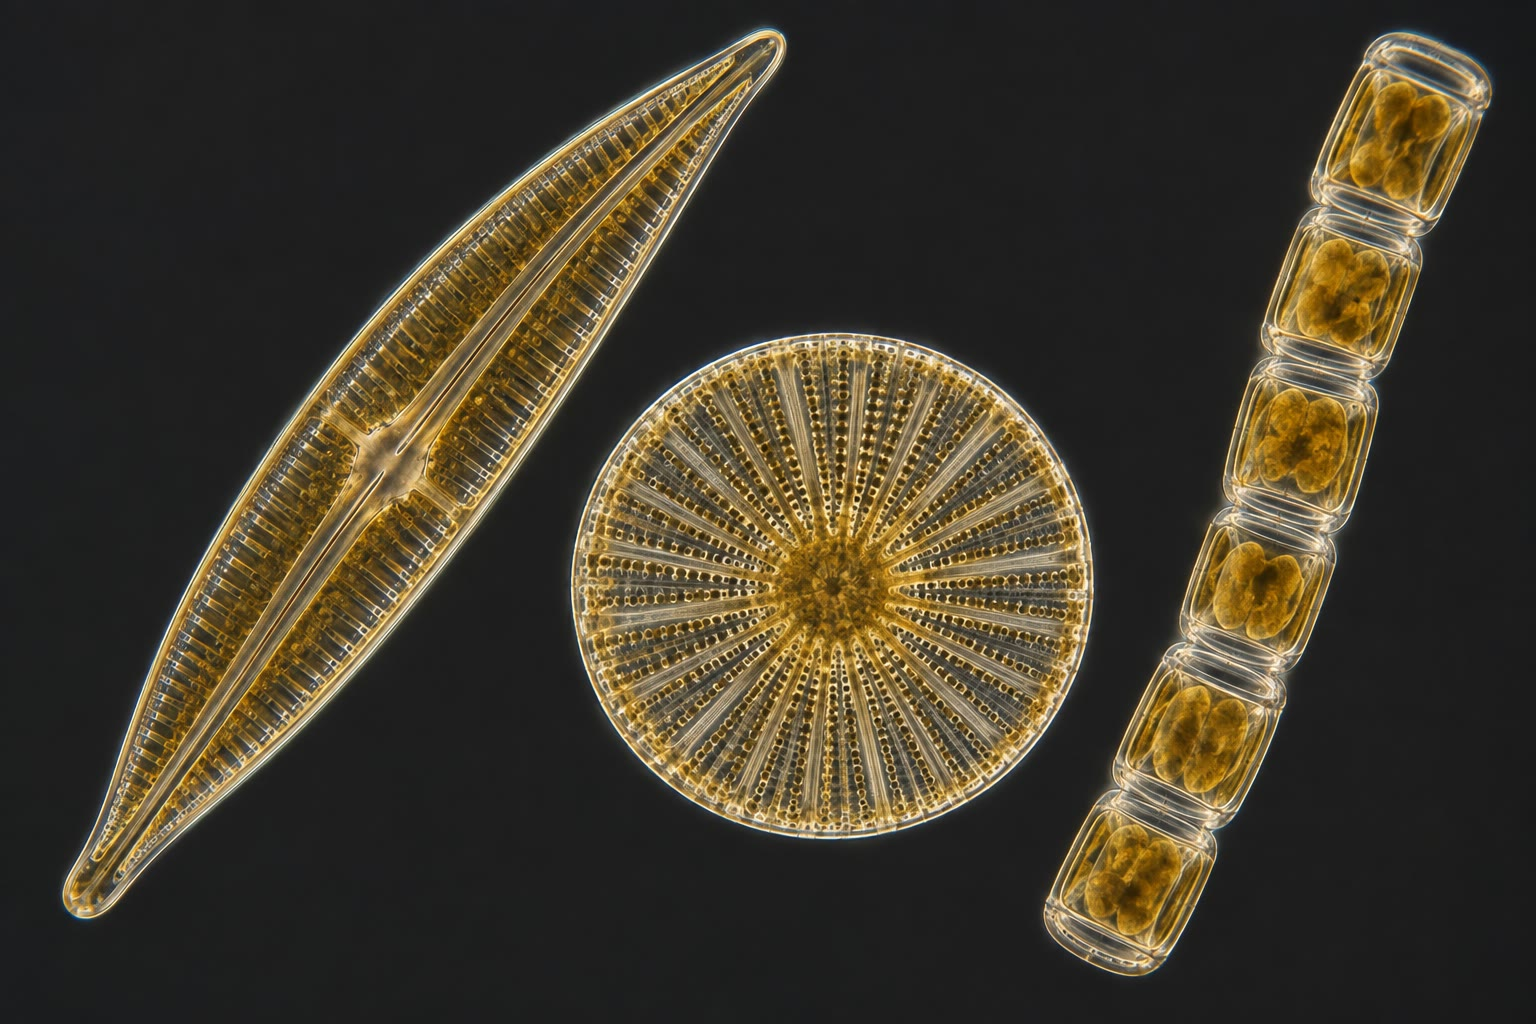
\includegraphics[width=0.6\linewidth]{images/book4/ai/b4-01-diatoms.jpg}

{\small دياتومات مرئية بالمجهر ذي الحقل المظلم: تعيش كل خلية في
قوقعة سيليسية ذات مصراعين، منقوشة بمسام تتبادل عبرها مع الماء.}
\end{omfigure}

\begin{definition}[أنماط التغذي]\label{def:b2:unicellular-diversity:nutrition}
\index{تغذٍّ بلعمي}\index{تغذٍّ تناضحي}\index{تغذٍّ مختلط}
يتغذى حقيقي النواة \omterm{def:b2:unicellular-diversity:unicellular}{وحيد الخلية} بإحدى ثلاث طرائق، أو باثنتين معًا.
\emph{التغذي الضوئي}: له صوانع خضراء يصنع بها مادته العضوية من
الضوء و$\mathrm{CO_2}$ (الطحالب الخضراء، والدياتومات، والسوطيات
الدوّارة). \emph{التغذي البلعمي}: يبتلع جسيمات --- بكتيريا،
وطلائعيات أخرى --- إلى فجوة غذائية تهضمها فيها إنزيمات جسيمية
حالّة (الأميبات، والهدبيات، والسوطيات المطوّقة).
\emph{التغذي التناضحي}: يمتص جزيئات منحلّة عبر غشائه، غالبًا بعد
إفراز إنزيمات إلى الخارج (الخمائر، وكثير من الطفيليات).
و\emph{مختلطات التغذي} مثل \emph{Euglena} تركّب ضوئيًا في الضوء
وتأكل في الظلام. أما بدائيات النوى فلا تستطيع البلعمة: الجدار
يمنعها، ولذلك لم يصر بدائي نواة قط مفترسًا بالابتلاع.
\end{definition}

\begin{proposition}[التنظيم التناضحي في الماء العذب]\label{prop:b2:unicellular-diversity:osmoregulation}
\index{فجوة متقلصة}
\omterm{def:b2:unicellular-diversity:protist}{طلائعي} الماء العذب أشد ملوحة في داخله (نحو \qty{100}{mmol/L} من
المنحلّات) من البركة (نحو \qty{1}{mmol/L})، وغشاؤه ينفذ الماء.
فالماء إذن يدخل باستمرار بالتناضح، بمعدل يتناسب مع مساحة السطح
وفرق الضغط التناضحي $\Delta\Pi = RT\,\Delta c$ --- أي نحو
\qty{2.4}{bar} عند الأرقام أعلاه. والخلية ذات الجدار تقاوم
بالامتلاء؛ أما الخلية العارية فكانت لتنتفخ وتنفجر في دقائق.
و\emph{\omterm{prop:b2:unicellular-diversity:osmoregulation}{الفجوة المتقلصة}} هي الجواب: خزان تغذيه قنوات شعاعية يمتلئ
بماء تضخه إليه ناقلات تدفعها البروتونات، ثم يتقلص فيطرد الماء عبر
ثقب، كل بضع ثوان إلى بضع دقائق. ويمرّر \emph{Paramecium} حجمه من
الماء كل نصف ساعة؛ أما أقاربه البحرية، في وسط بملوحتها، فلا \omterm{prop:b2:unicellular-diversity:osmoregulation}{فجوة
متقلصة} لها أصلًا.
\end{proposition}

\section{فيزياء سابح صغير}

\begin{proposition}[الحياة عند عدد رينولدز الصغير]\label{prop:b2:unicellular-diversity:reynolds}
\index{عدد رينولدز}
\emph{\omterm{prop:b2:unicellular-diversity:reynolds}{عدد رينولدز}} $Re = \rho v L/\eta$ يقارن قوى العطالة بالقوى
اللزجة عند جسم قياسه $L$ يتحرك بسرعة $v$ في مائع كثافته $\rho$
ولزوجته $\eta$. وهو عند سابح بشري نحو $10^6$؛ وعند
\emph{Paramecium} (\qty{200}{\micro m}، \qty{1}{mm/s}) يساوي 0.2،
وعند بكتيريا $10^{-5}$. ودون $Re \approx 1$ تصير العطالة عديمة
الأثر: فالخلية التي تكفّ عن الضرب تقف خلال نانومتر، والماء يشبه
شرابًا ثخينًا، والحركة الترادفية (الضربة نفسها ذهابًا وإيابًا) لا
تعطي انزياحًا صافيًا. ولذلك يستعمل السابحون الصغار ضربات غير
ترادفية: الحلزون الدوّار في السوط البكتيري، والضربة اللامتناظرة في
الهدب (ضربة قوة متيبسة، ثم استرجاع ملتفّ)، وضربة الصدر عند
\emph{Chlamydomonas}.
\end{proposition}

\begin{theorem}[قانون ستوكس والترسّب]\label{thm:b2:unicellular-diversity:stokes}
\index{قانون ستوكس}
كرة نصف قطرها $r$ وكثافتها $\rho_{\text{الخلية}}$ تتحرك ببطء في مائع
لزوجته $\eta$ تحس بقوة جرّ $F = 6\pi\eta r v$. وإذا تُركت وشأنها في
ماء كثافته $\rho$ هبطت بالسرعة الحدية
\[
v_s = \frac{2\,r^2\,(\rho_{\text{الخلية}} - \rho)\,g}{9\eta},
\]
وهي تتناسب مع مربع نصف القطر: فخلية أكبر بعشر مرات تهبط أسرع بمئة
مرة. ولهذا كانت العوالق النباتية صغيرة، ولهذا تحمل الدياتومات
أشواكًا وقطيرات زيت، ولهذا يهبط \emph{Chlamydomonas} الذي يكفّ عن
السباحة خارج الضوء في أيام قليلة.
\end{theorem}
\begin{proof}
عند السرعة الحدية توازن قوة الجرّ الوزن الظاهري (الوزن ناقص قوة
الطفو): $6\pi\eta r v_s = \tfrac{4}{3}\pi r^3
(\rho_{\text{الخلية}} - \rho) g$. وحلّ هذه من أجل $v_s$ يعطي الصيغة.
أما قانون الجرّ نفسه فمشتق في سلسلة الفيزياء من أجل
$Re \ll 1$؛ وهو هنا مسلّم به.
\end{proof}

\begin{example}[سقوط دياتوم]\label{ex:b2:unicellular-diversity:fall}
دياتوم مركزي نصف قطره \qty{10}{\micro m}، أكثف من ماء البحر بمقدار
\qty{100}{kg/m^3} ($\eta = \qty{1e-3}{Pa.s}$)، يهبط بسرعة
$v_s = 2\times 10^{-10}\times 100\times 9.81/(9\times 10^{-3}) =
\qty{2.2e-5}{m/s}$، أي نحو \qty{2}{m} في اليوم: فهو يغادر الطبقة
المضاءة البالغة \qty{50}{m} في أقل من شهر. وتبقى جمهراته لأن
الاضطراب يقلّب الماء، ولأن قطيرات الزيت وكثافة منخفضة تقلّصان
$\rho_{\text{الخلية}} - \rho$، ولأن خلية تهبط وتنقسم في الطريق تخلّف
ذرية تُرفع من جديد.
\end{example}

\begin{omfigure}
\begin{tikzpicture}
\begin{axis}[
  width=0.8\linewidth, height=6.0cm,
  axis x line=bottom, axis y line=left,
  xmode=log, ymode=log,
  xmin=0.5, xmax=200, ymin=1e-3, ymax=1e4,
  xlabel={نصف القطر (\unit{\micro m})}, ylabel={سرعة الهبوط (\unit{\micro m/s})},
  xlabel style={font=\small, at={(axis description cs:0.5,-0.1)}, anchor=north},
  ylabel style={font=\small},
  tick label style={font=\small},
  clip=false,
]
\addplot[very thick, omDef, domain=0.5:200, samples=40] {0.218*x^2};
\addplot[only marks, mark=*, mark size=1.8pt, omThm] coordinates {(1,0.218) (10,21.8) (100,2180)};
\node[font=\scriptsize, anchor=west] at (axis cs:1.15,0.218) {بكتيريا};
\node[font=\scriptsize, anchor=west] at (axis cs:11.5,21.8) {دياتوم};
\node[font=\scriptsize, anchor=east] at (axis cs:85,2180) {طلائعي كبير};
\end{axis}
\end{tikzpicture}

{\small سرعة الهبوط \omterm{thm:b2:unicellular-diversity:stokes}{بقانون ستوكس} بدلالة نصف القطر، عند خلايا أكثف
من الماء بمقدار \qty{100}{kg/m^3}. والميل 2 على محاور لوغاريتمية هو
قانون $r^2$: فالبكتيريا تهبط سنتيمترًا في اليوم، \omterm{def:b2:unicellular-diversity:protist}{والطلائعي} الكبير
مترين في الساعة.}
\end{omfigure}

\section{التكاثر والجنس في خلية واحدة}

\begin{definition}[أنماط الانقسام]\label{def:b2:unicellular-diversity:division}
\index{انشطار ثنائي}\index{تبرعم}\index{انشطار متعدد}
يتكاثر \omterm{def:b2:unicellular-diversity:unicellular}{الكائن وحيد الخلية} بالانقسام. \emph{الانشطار الثنائي}: تنمو
الخلية إلى ضعف قياسها ثم تنشطر إلى بنتين متساويتين (البكتيريا،
و\emph{Paramecium}، و\emph{Amoeba}). \emph{التبرعم}: تنمو بنت
صغيرة من الأم ثم تنفصل (الخميرة؛ وتحتفظ الأم بندبة وتستطيع أن
تبرعم نحو عشرين مرة). \emph{الانشطار المتعدد}: تكبر الخلية، ثم
تنقسم عدة مرات متتابعة سريعًا داخل جدار الأم فتطلق 4 أو 8 أو 16
بنتًا أو أكثر دفعة واحدة (\emph{Chlamydomonas}، وطفيلي الملاريا في
كرية حمراء). وفي ظروف ثابتة ينمو عدد الخلايا أسّيًا،
$N(t) = N_0\,2^{t/T}$ حيث $T$ هو \emph{زمن الجيل}\index{زمن الجيل}:
عشرون دقيقة عند \emph{E.~coli} في وسط غني، ويوم عند كثير
من الطحالب، وأسبوع عند بعض الهدبيات. (ويُعالَج النمو بدلالة الغذاء
في \cref{ch:b2:microbial-metabolism}.)
\end{definition}

\begin{proposition}[جنس بلا تكاثر: الاقتران عند \emph{Paramecium}]\label{prop:b2:unicellular-diversity:conjugation}
\index{اقتران!هدبيات}
يلتحم فردان من \emph{Paramecium} من نمطي تزاوج متتامّين بسطحيهما
الفمويين. وفي كل منهما تخضع النواة الصغيرة الثنائية الصيغة للتقسم
المنصّف فتعطي أربع نوى فردية الصيغة، تنحلّ ثلاث منها؛ ثم تنقسم
الباقية تقسمًا خيطيًا إلى نواة ثابتة وأخرى مهاجرة، وتتبادل الخليتان
نواتيهما المهاجرتين عبر الوصل. ثم تدمج كل خلية نواتها الثابتة مع
التي تلقّتها، ويفترق الشريكان، ولكل منهما نواة صغيرة ثنائية الصيغة
جديدة بالنمط الوراثي نفسه الذي لشريكه. وتتحلل النواة الكبيرة
القديمة وتُبنى واحدة جديدة من النواة الصغيرة الجديدة. ولم تُصنع
خلية جديدة: فالاقتران خلط وراثي --- تقسم منصّف وإلقاح،
\cref{ch:b2:meiosis-heredity} --- منفصل عن التكاثر. أما الاقتران
البكتيري، الذي ينقل بلازميدًا في اتجاه واحد من واهب إلى متلقٍّ،
فعملية أخرى تحمل الاسم نفسه
(\cref{ch:b2:genome-diversification}).
\end{proposition}

\begin{omfigure}
\begin{tikzpicture}[every node/.style={font=\scriptsize}]
  \foreach \i/\x in {0/0,1/3.6,2/7.2,3/10.8} {
    \draw[thick, fill=omProp!8] (\x,0.55) ellipse (1.0 and 0.5);
    \draw[thick, fill=omProp!8] (\x,-0.55) ellipse (1.0 and 0.5);
  }
  % stage 0: two cells, diploid micronuclei 2n
  \fill[omDef!90!black] (0,0.55) circle (0.12); \node[right] at (0.15,0.55) {$2n$};
  \fill[omDef!90!black] (0,-0.55) circle (0.12); \node[right] at (0.15,-0.55) {$2n$};
  \node[below, align=center] at (0,-1.15) {خليتان تلتحمان};
  % stage 1: meiosis, 4 haploid, 3 degenerate
  \foreach \dy in {0.55,-0.55} {
    \fill[omDef!90!black] (3.6-0.3,\dy+0.15) circle (0.08);
    \fill[gray!60] (3.6+0.1,\dy+0.2) circle (0.06);
    \fill[gray!60] (3.6+0.3,\dy-0.05) circle (0.06);
    \fill[gray!60] (3.6-0.1,\dy-0.25) circle (0.06);
  }
  \node[below, align=center] at (3.6,-1.15) {تقسم منصّف:\\4 نوى فردية الصيغة،\\تنحل ثلاث منها};
  % stage 2: mitosis, exchange
  \foreach \dy in {0.55,-0.55} {
    \fill[omDef!90!black] (7.2-0.35,\dy) circle (0.08);
    \fill[omThm] (7.2+0.35,\dy) circle (0.08);
  }
  \draw[->, thick, omThm] (7.55,0.45) -- (7.55,-0.45);
  \draw[->, thick, omThm] (6.85,-0.45) -- (6.85,0.45);
  \node[below, align=center] at (7.2,-1.15) {تقسم خيطي؛ النوى\\المهاجرة (بالأحمر)\\تُتبادل};
  % stage 3: fusion 2n
  \fill[omDef!90!black] (10.8,0.55) circle (0.12); \node[right] at (10.95,0.55) {$2n$};
  \fill[omDef!90!black] (10.8,-0.55) circle (0.12); \node[right] at (10.95,-0.55) {$2n$};
  \node[below, align=center] at (10.8,-1.15) {إلقاح:\\نوى ثنائية الصيغة\\جديدة متماثلة؛ وتفترق الخليتان};
  \foreach \x in {1.3,4.9,8.5} \draw[->, thick, gray] (\x,0) -- (\x+1.0,0);
\end{tikzpicture}

{\small الاقتران عند \emph{Paramecium}. تتبادل خليتان نوى فردية
الصيغة ثم تفترقان، وكل منهما تحمل نواة صغيرة ثنائية الصيغة
معاد تركيبها؛ ولم يتغير عدد الخلايا.}
\end{omfigure}

\section{نحو تعدد الخلايا}

\begin{proposition}[السلسلة الفولفوكسية]\label{prop:b2:unicellular-diversity:volvox}
\index{Volvox@\emph{Volvox}}\index{تعدد الخلايا، نشأة}
تعرض سلالة واحدة من الطحالب الخضراء، في أنواع حية، الخطوات من خلية
واحدة إلى جسم. أما \emph{Chlamydomonas} فيعيش وحده. و\emph{Gonium}
صفيحة مسطحة من 4 إلى 16 خلية متماثلة تسبح معًا. و\emph{Pandorina}
و\emph{Eudorina} كرتان جوفاوان من 16 إلى 32 خلية، كلها متشابهة
بعد، وكل منها قادرة على تأسيس مستعمرة جديدة. وعند \emph{Pleodorina}
خلايا صغيرة تسبح فقط ولا تنقسم أبدًا. و\emph{Volvox} كرة من
\num{500} إلى \num{50000} خلية جسدية صغيرة مسوّطة، ستموت مع
المستعمرة، تحيط بحفنة من خلايا إنتاشية كبيرة (غونيديات) تنقسم
فتكوّن كرات بنات داخل الأم. فقد ظهرت الخلايا الجسدية والإنتاشية:
وهذه عتبة تعدد الخلايا، عُبرت في هذه السلالة قبل نحو \num{200}
مليون سنة، وعُبرت مستقلةً خمسًا وعشرين مرة على الأقل في مواضع أخرى
من شجرة الحياة --- عند الحيوانات والنباتات والفطريات والطحالب
البنية والطحالب الحمراء وعدة مجموعات بكتيرية.
\end{proposition}
\begin{proof}[شواهد]
التصنيف الجزيئي للطحالب الفولفوكسية، المبني على عشرات المورّثات،
يضع \emph{Chlamydomonas} في القاعدة و\emph{Volvox} عند الأطراف،
والأشكال المستعمرية بينهما، وعدد الخلايا يتزايد على امتداد الفروع؛
ومورثوم \emph{Volvox carteri} (2010) لا يختلف عن مورثوم
\emph{Chlamydomonas} إلا ببضع مئات من المورّثات، أكثرها مورّثات
الحشوة خارج الخلوية التي تمسك الخلايا، ومورّثات المنظِّمات التي
تُسكت الانقسام في الخلايا الجسدية. فالانتقال احتاج مادة وراثية
جديدة قليلة إلى حد لافت.
\end{proof}

\begin{omfigure}
\begin{tikzpicture}[every node/.style={font=\scriptsize}]
  % Chlamydomonas
  \draw[thick, fill=omProp!25] (0,0) circle (0.22);
  \node[below=0.35cm, align=center] at (0,0) {\emph{Chlamydomonas}\\خلية واحدة};
  % Gonium plate
  \begin{scope}[xshift=2.2cm]
    \foreach \x in {-0.3,0,0.3} \foreach \y in {-0.3,0,0.3} \draw[thick, fill=omProp!25] (\x,\y) circle (0.14);
    \draw[gray, dashed] (-0.55,-0.55) rectangle (0.55,0.55);
    \node[below=0.7cm, align=center] at (0,0) {\emph{Gonium}\\صفيحة من 8--16};
  \end{scope}
  % Eudorina ball
  \begin{scope}[xshift=4.5cm]
    \draw[gray, dashed] (0,0) circle (0.6);
    \foreach \a in {0,45,...,315} \draw[thick, fill=omProp!25] (\a:0.55) circle (0.13);
    \draw[thick, fill=omProp!25] (0,0.1) circle (0.13);
    \node[below=0.7cm, align=center] at (0,0) {\emph{Eudorina}\\كرة من 32،\\كلها متشابهة};
  \end{scope}
  % Pleodorina
  \begin{scope}[xshift=7.4cm]
    \draw[gray, dashed] (0,0) circle (0.7);
    \foreach \a in {0,30,...,330} \draw[thick, fill=omProp!25] (\a:0.62) circle (0.09);
    \foreach \a in {60,180,300} \draw[thick, fill=omProp!60] (\a:0.62) circle (0.14);
    \node[below=0.8cm, align=center] at (0,0) {\emph{Pleodorina}\\بعض الخلايا\\تسبح فقط};
  \end{scope}
  % Volvox
  \begin{scope}[xshift=10.6cm]
    \draw[thick, fill=omProp!6] (0,0) circle (0.95);
    \foreach \a in {0,12,...,348} \fill[omProp!70] (\a:0.9) circle (0.035);
    \foreach \a in {0,12,...,348} \fill[omProp!50] (\a:0.72) circle (0.03);
    \foreach \p in {(0.25,0.2),(-0.3,-0.25),(0.1,-0.4),(-0.2,0.35)} \draw[thick, omThm, fill=omThm!40] \p circle (0.13);
    \node[below=1.05cm, align=center] at (0,0) {\emph{Volvox}\\آلاف الخلايا الجسدية\\وقليل من الخلايا الإنتاشية (بالأحمر)};
  \end{scope}
  \foreach \x in {0.5,3.0,5.3,8.3} \draw[->, gray] (\x,0) -- (\x+0.6,0);
\end{tikzpicture}

{\small السلسلة الفولفوكسية: خلية مفردة، ثم صفيحة، ثم كرة جوفاء من
خلايا متماثلة، ثم كرة تخلّت فيها بعض الخلايا عن الانقسام، ثم
\emph{Volvox} حيث تحيط آلاف الخلايا الجسدية الفانية بقليل من
الخلايا الإنتاشية.}
\end{omfigure}

\begin{omfigure}
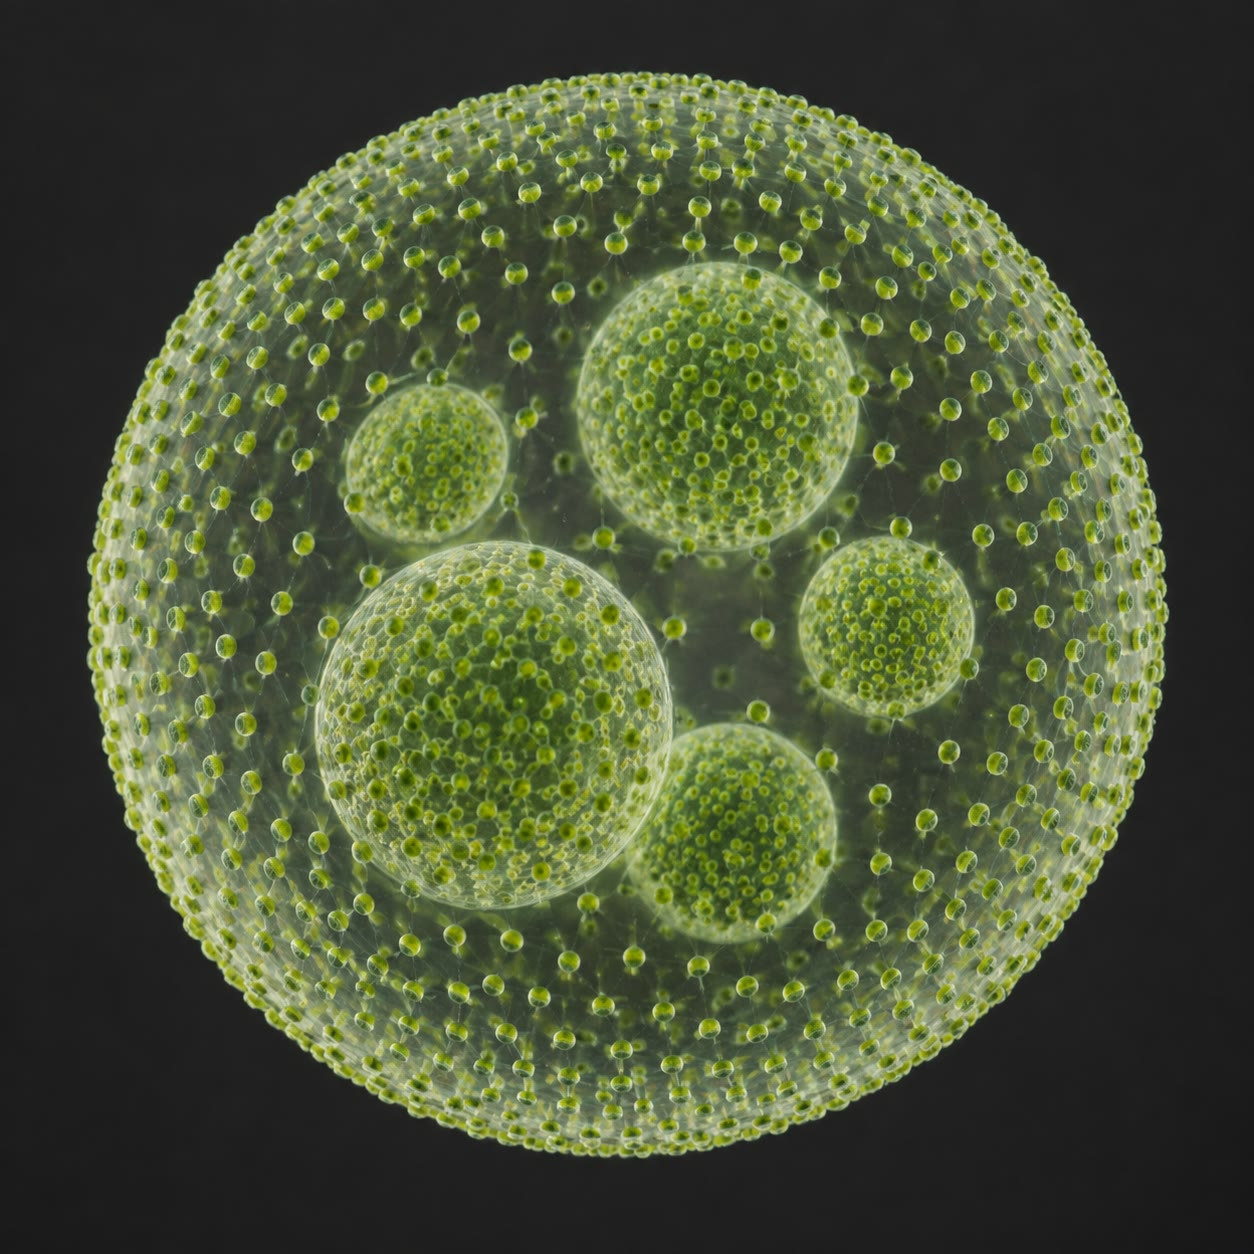
\includegraphics[width=0.55\linewidth]{images/book4/ai/b4-01-volvox.jpg}

{\small مستعمرة \emph{Volvox}: كرة خضراء جوفاء من خلايا مسوّطة،
وفي داخلها مستعمرات بنات تنمو.}
\end{omfigure}

\begin{remark}[لماذا يُقسَّم العمل؟]\label{rem:b2:unicellular-diversity:whydivide}
لا تستطيع الخلية في هذه الطحالب أن تسبح وتنقسم في آن واحد: فالأجسام
القاعدية التي ترسو عليها الأسواط لازمة لتنظيم المغزل. فالخلية
المفردة تناوب بين الأمرين؛ والمستعمرة الصغيرة تحتمل أن تكفّ عن
السباحة بينما تنقسم خلاياها كلها؛ أما المستعمرة الكبيرة فكانت
لتهبط خارج الضوء (\omterm{thm:b2:unicellular-diversity:stokes}{قانون ستوكس}،
\cref{thm:b2:unicellular-diversity:stokes}) خلال الساعات التي
يستغرقها انقسامها. فوراء قياس معين، يستحق إبقاءُ بعض الخلايا سابحة
بينما تنقسم غيرها ثمنَ خسارة ذريتها --- وهكذا يولد الجسد. والسوطيات
المطوّقة، وهي سوطيات خليتها نسخة من خلية الإسفنج الغذائية، تُظهر
الخطوات الأولى نفسها على الفرع الذي أفضى إلى الحيوانات.
\end{remark}

\section{تمارين}

\begin{exercise}[$\star$]\label{exo:b2:unicellular-diversity:1}
عرّف \omterm{def:b2:unicellular-diversity:unicellular}{وحيد الخلية} والمستعمري \omterm{def:b2:unicellular-diversity:unicellular}{وعديد الخلايا}، وضع \emph{E.~coli}
و\emph{Gonium} و\emph{Volvox} وخلية خميرة في الصنف الصحيح مع
التعليل.
\end{exercise}

\begin{exercise}[$\star$]\label{exo:b2:unicellular-diversity:2}
احسب \omterm{prop:b2:unicellular-diversity:surface}{نسبة السطح إلى الحجم} عند مكوّر نصف قطره \qty{0.5}{\micro m}
وعند \omterm{def:b2:unicellular-diversity:protist}{طلائعي} كروي نصف قطره \qty{50}{\micro m}. فأيهما يتنفس أسرع
لكل وحدة من السيتوبلازم، ولماذا؟
\end{exercise}

\begin{exercise}[$\star$]\label{exo:b2:unicellular-diversity:3}
اذكر ثلاثة فروق بنيوية بين بكتيريا وحقيقي نواة \omterm{def:b2:unicellular-diversity:unicellular}{وحيد الخلية}، وأمرًا
واحدًا لا تستطيعه البكتيريا وتستطيعه الأميبا.
\end{exercise}

\begin{exercise}[$\star$]\label{exo:b2:unicellular-diversity:4}
سمّ وظيفة كل بنية من بنى \emph{Paramecium} الآتية: الأهداب،
والميزاب الفموي، والفجوة الغذائية، \omterm{prop:b2:unicellular-diversity:osmoregulation}{والفجوة المتقلصة}، والنواة
الكبيرة، والنواة الصغيرة.
\end{exercise}

\begin{exercise}[$\star\star$]\label{exo:b2:unicellular-diversity:5}
مع $D = \qty{5e-10}{m^2/s}$ لمستقلَب في السيتوبلازم، كم يستغرق
الانتشار عبر بكتيريا قياسها \qty{1}{\micro m} وعبر أميبا قياسها
\qty{500}{\micro m}؟ وعلّق على ما يجب على الأميبا أن تفعله ولا يجب
على البكتيريا.
\end{exercise}

\begin{exercise}[$\star\star$]\label{exo:b2:unicellular-diversity:6}
احسب \omterm{prop:b2:unicellular-diversity:reynolds}{عدد رينولدز} عند \emph{Paramecium} (\qty{200}{\micro m}،
\qty{1}{mm/s})، وعند بكتيريا (\qty{2}{\micro m}،
\qty{20}{\micro m/s})، وعند سابح بشري (\qty{2}{m}، \qty{1}{m/s})،
مع $\rho = \qty{1000}{kg/m^3}$ و$\eta = \qty{1e-3}{Pa.s}$. ولماذا
يستطيع السابح أن ينزلق بعد ضربة ولا تستطيع البكتيريا؟
\end{exercise}

\begin{exercise}[$\star\star$]\label{exo:b2:unicellular-diversity:7}
دياتوم نصف قطره \qty{10}{\micro m} أكثف من الماء بمقدار
\qty{100}{kg/m^3}. احسب سرعة هبوطه وزمن سقوطه عبر \qty{50}{m}.
وبأي عامل يتغير الزمن إذا نصّفت الخلية نصف قطرها؟ وإذا قلّصت فائض
كثافتها إلى \qty{20}{kg/m^3}؟
\end{exercise}

\begin{exercise}[$\star\star$]\label{exo:b2:unicellular-diversity:8}
مثّل \emph{Paramecium} بإهليلجي أنصاف محاوره \num{100} و\num{25}
و\qty{25}{\micro m} ($V = \tfrac{4}{3}\pi abc$). وهو يطرد حجمه من
الماء كل \qty{30}{min}. احسب وارد الماء
بوحدة \unit{\micro m^3/s} وباللترات في الثانية.
\end{exercise}

\begin{exercise}[$\star\star$]\label{exo:b2:unicellular-diversity:9}
يتضاعف تركيز مادة جاذبة على امتداد \qty{1}{mm}. فما الفرق النسبي
بين طرفي بكتيريا قياسها \qty{1}{\micro m}؟ وما الفرق بين بداية شوط
مدته \qty{1}{s} بسرعة \qty{20}{\micro m/s} ونهايته؟ ولمّا كان عدّ
$N$ جزيئة يحمل خطأ نسبيًا قدره نحو $1/\sqrt{N}$، فسّر لماذا تقارن
البكتيريا الأزمنة لا الجانبين.
\end{exercise}

\begin{exercise}[$\star\star\star$]\label{exo:b2:unicellular-diversity:10}
\emph{Thiomargarita namibiensis} بكتيريا كبريتية كروية قطرها
\qty{500}{\micro m} وسيتوبلازمها قشرة ثخنها \qty{2}{\micro m} حول
فجوة من النترات. احسب نسبة سطحها إلى حجمها \emph{السيتوبلازمي}
وقارنها بما عند \emph{E.~coli} (أسطوانة نصف قطرها \qty{0.5}{\micro m}؛
أهمل الطرفين). وفسّر كيف تتيح لها الفجوة أن تكون بهذا الكبر، وما
فائدة النترات.
\end{exercise}

\begin{exercise}[$\star\star\star$]\label{exo:b2:unicellular-diversity:11}
في \emph{Volvox} لا تنقسم الخلايا الجسدية أبدًا وتموت مع المستعمرة.
باستعمال قيد التسويط \omterm{thm:b2:unicellular-diversity:stokes}{وقانون ستوكس}، فسّر لماذا تستحق هذه الخلايا
الاقتناء في مستعمرة من \num{10000} خلية دون مستعمرة من 16، ولماذا
تكون الخلايا الإنتاشية أكبر خلايا الكرة.
\end{exercise}

\begin{exercise}[$\star\star\star$]\label{exo:b2:unicellular-diversity:12}
«\omterm{def:b2:unicellular-diversity:protist}{الطلائعيات} درجة لا فرع حيوي.» اشرح هذا الفرق بالسلالات المذكورة في
هذا الفصل، وقل لماذا تصدق العبارة نفسها على «بدائيات النوى» ولا
تصدق على «الزراقم».
\end{exercise}

\section{مسألة: قطرة من ماء بركة}

\begin{problem}[{مسألة نهاية الأسبوع --- عينة من ماء بركة تُعدّ
وتُنمّى وتُحلّل من جهة الفيزياء التي تحكم خلاياها، وتنتهي إلى
ميزان الماء والطاقة عند طحلب أخضر}]
\label{pb:b2:unicellular-diversity:1}
بركة حجمها \qty{1000}{m^3} تؤخذ منها عينة في الربيع. وتحت المجهر،
تبين خانة عدّ شبكتها تغطي \qty{1}{mm}$\times$\qty{1}{mm} تحت
ساترة مرفوعة \qty{0.1}{mm} فوقها 24 خلية من
\emph{Chlamydomonas} (كرات نصف قطرها \qty{5}{\micro m}،
كثافتها \qty{1050}{kg/m^3}). خذ $\rho = \qty{1000}{kg/m^3}$،
و$\eta = \qty{1e-3}{Pa.s}$، و$g = \qty{9.81}{m/s^2}$، و$R =
\qty{8.314}{J/mol/K}$، و$T = \qty{293}{K}$، و$D = \qty{1.9e-9}{m^2/s}$
من أجل $\mathrm{CO_2}$ في الماء.

\medskip
\noindent\textbf{الجزء الأول --- العدّ.}
\begin{enumerate}
  \item احسب حجم الماء تحت الشبكة، بالميكرولترات.
  \item استنتج كثافة \emph{Chlamydomonas} في البركة، بعدد الخلايا
        في المليلتر.
  \item احسب حجم خلية واحدة ونسبة سطحها إلى حجمها.
  \item ما الكسر الذي تشغله هذه الخلايا من حجم ماء البركة؟
  \item كم خلية من \emph{Chlamydomonas} تضم البركة؟
  \item يوجد أيضًا زُراق خيطي. اذكر صفتين مرئيتين تحت المجهر
        تميزانه عن الطحلب.
\end{enumerate}

\medskip
\noindent\textbf{الجزء الثاني --- النمو.}
تُحفظ العينة في الضوء وتُعدّ ثانيةً بعد \qty{48}{h}:
\num{384} خلية تحت الشبكة.
\begin{enumerate}[resume]
  \item احسب \omterm{def:b2:unicellular-diversity:division}{زمن الجيل} $T$.
  \item احسب ثابت معدل النمو $k$ في $N = N_0 e^{kt}$، بوحدة
        \unit{h^{-1}}.
  \item كم يلزم جمهرة البركة من الزمن لتبلغ \qty{1e8}{} خلية في
        المليلتر بهذا المعدل؟
  \item اذكر ثلاثة أسباب تمنع بلوغ ذلك.
  \item إذا لم تنمُ الخلايا إلا خلال \qty{12}{h} من ضوء النهار ولم
        تنمُ ليلًا البتة، فكم تستغرق الزيادة نفسها؟
  \item ينقسم \emph{Chlamydomonas} \omterm{def:b2:unicellular-diversity:division}{بالانشطار المتعدد}، فيطلق 4 أو 8
        أو 16 بنتًا دفعة واحدة. فسّر لماذا يظل \omterm{def:b2:unicellular-diversity:division}{زمن الجيل} معرّفًا
        تعريفًا جيدًا من العدّ رغم ذلك.
\end{enumerate}

\medskip
\noindent\textbf{الجزء الثالث --- فيزياء الخلية.}
\begin{enumerate}[resume]
  \item احسب \omterm{prop:b2:unicellular-diversity:reynolds}{عدد رينولدز} عند خلية تسبح بسرعة
        \qty{100}{\micro m/s}.
  \item خلية كتلتها $m$ تكفّ عن ضرب أسواطها تنزلق مسافة
        $mv/(6\pi\eta r)$. احسبها.
  \item احسب سرعة هبوط خلية كفّت عن السباحة.
  \item قارن زمن الهبوط \qty{1}{m} بزمن السباحة صعودًا
        \qty{1}{m}.
  \item تضم البركة \qty{10}{\micro mol/L} من
        $\mathrm{CO_2}$ المنحلّ. احسب أقصى وارد بالانتشار من
        $\mathrm{CO_2}$ إلى خلية، بالجزيئات في الثانية.
  \item تحوي الخلية \qty{100}{pg} من الكربون وتضاعفها في جيل
        واحد. احسب متوسط طلبها من الكربون بالجزيئات في الثانية،
        ونسبة الوارد إلى الطلب.
  \item أعد المقارنة من أجل خلية افتراضية نصف قطرها
        \qty{50}{\micro m} بكثافة الكربون نفسها. واستنتج.
\end{enumerate}

\medskip
\noindent\textbf{الجزء الرابع --- الماء والطاقة.}
يحوي السيتوبلازم \qty{100}{mmol/L} من المنحلّات، والبركة
\qty{1}{mmol/L}. والناقلية المائية للغشاء $L_p =
\qty{1e-14}{m.s^{-1}.Pa^{-1}}$ (تدفق حجم الماء لكل وحدة مساحة لكل
وحدة فرق ضغط). وحلمهة ATP واحد تعطي
\qty{50}{kJ/mol}؛ وتثبيت ذرة كربون واحدة يكلف ثلاثة ATP.
\begin{enumerate}[resume]
  \item احسب فرق الضغط التناضحي عبر الغشاء.
  \item احسب حجم الماء الداخل إلى الخلية في الثانية، بوحدة
        \unit{\micro m^3/s}.
  \item لولا \omterm{prop:b2:unicellular-diversity:osmoregulation}{فجوة متقلصة}، كم كانت الخلية تستغرق لتضاعف حجمها؟
  \item احسب أصغر استطاعة لازمة لطرد هذا الماء ضد الضغط التناضحي.
  \item حوّلها إلى جزيئات ATP في الثانية وقارنها بما تنفقه الخلية
        من ATP على تثبيت الكربون (السؤال 18).
  \item اذكر النتيجة: وارد الماء إلى الخلية، والزمن الذي كانت
        ستنفجر فيه، وكسر طاقتها الذي يكلفه بقاؤها جافة.
\end{enumerate}
\end{problem}
